% use the option blindreview to mask the author details for blind review submission
% remove the blinereview option to make the author information visible
\documentclass[fleqn, 10pt, twoside]{IOEGC}
\usepackage{listings}

\usepackage{svg}
\usepackage{caption}
\usepackage{subcaption}
\usepackage{graphicx}
\usepackage{afterpage}
\usepackage{float}
\lstdefinestyle{mystyle}{
    language=Python,
    basicstyle=\small\ttfamily,,
    keywordstyle=\color{blue},
    commentstyle=\color{green},
    stringstyle=\color{purple},
    showstringspaces=false,
    numbers=left,
    numberstyle=\tiny,
    numbersep=5pt,
    breaklines=true,
    breakatwhitespace=true,
    tabsize=2
}
\hypersetup
{
    pdfauthor   = {Zishan Siddique, Sandip Pariyar, Venus Bastola, Sushant Phagu, Binay lal Shrestha, Pravin Sangroula},	% Edit with actual author names 
}

\begin{document}

\maketitle
\thispagestyle{firstpage}

\section{Introdution}
Nepal is a land of unparalleled biodiversity with 208 species of mammals \cite{r1}, 142 species of reptiles \cite{r2}, and more than 873 species of birds \cite{r3}. The diverse wildlife, including endangered species found here, are testament to the country’s commitment to conservation. However, with the increasing challenges posed
by habitat loss, poaching, and climate change, preserving Nepal’s wildlife heritage demands innovative and technologically advanced approaches.
This project provides a basic template for creating solutions to bolster wildlife conservation efforts in Nepal.
\par
Vision can be sufficient for some species that are of adequate size but vision alone can miss many opportunities for identification and classification. For this reason, we have used two models i.e. vision and audio for a broader scope.
The paper is structured as follows:
\begin{itemize}
	\item Earlier approaches for our objectives are discussed in Section 2.
	\item The datasets used and their metainformation are explained in Section 3.
	\item Our approach for the proposed system is elaborated in Section 4.
	\item The results of our solution are explained in Section 5.
	\item Finally, the complete project is concluded with a brief paragraph in Section 6.
\end{itemize}


\section{Background and Related Works}
There have been many instances of work done for wildlife. In 2017, Nguyen et al.\cite{r4} worked on a monitoring system for animals in South-central Victoria, Australia with appreciable results. HOW?
\par
Gautam et al. 2023 \cite{r5} worked on the classification of birds based on audio data of 44 species found in Nepal. Their work was based on Mel Spectogram features which are often termed "pictures of a sound". Mel Spectogram and MFCC (Mel-Frequency Cepstral Coefficients) were used for feature extraction of audio data which was used to train a Convolutional Neural Network.
\par
In 2021, Qi et al. \cite{r6} worked on image recognition in Animal Husbandry. They applied super pixel-based image segmentation and SIFT algorithm to complete image segmentation and feature extraction which was later modeled using Convolutional Neural Network and SVM for classification.
\par
We propose an integrated system of using both audio and video. The audio is used as it is with some pre-processing and the video is broken into frames which are fed to the image classifier model.

\section{Dataset Analysis}
As two mediums vision and audio are being used for classification of animals, two different datasets comprising of labeled images and labeled audio are required.
The image dataset has a total of 44 classes. Of the 44 classes, there are 31 mammals, 9 birds, and 4 reptiles. Moreover, we couldn’t find research-grade audio data for groups of animals other than birds. Thus, the audio model comprises 23 classes of birds all found in Nepal.
\subsection{Image Data from iNaturalist}
iNaturalist is an online social network of people sharing biodiversity information. It has a large size of data which includes images, audio, and video of large number of species found around the world. The data is collected by users who submit it to the site under the public domain, Creative Commons, or with all rights reserved. iNaturalist encourages its users to opt for more open licenses like Creative Commons for the research community.We collected a total of 38,442 images spanning across 44 species all found in Nepal. As the data contained some anomalous images, we had to manually remove them. After the cleaning step, the data was preprocessed as per the Efficient Net Model for better training. Of the 38,442 images collected, 50 images from each class were used as test datasets.
API provided by iNaturalist was used for downloading the data. The bar chart in Figure \ref{image-file-count-animal} shows the frequency of each class of image.

\begin{figure}
	\centering
	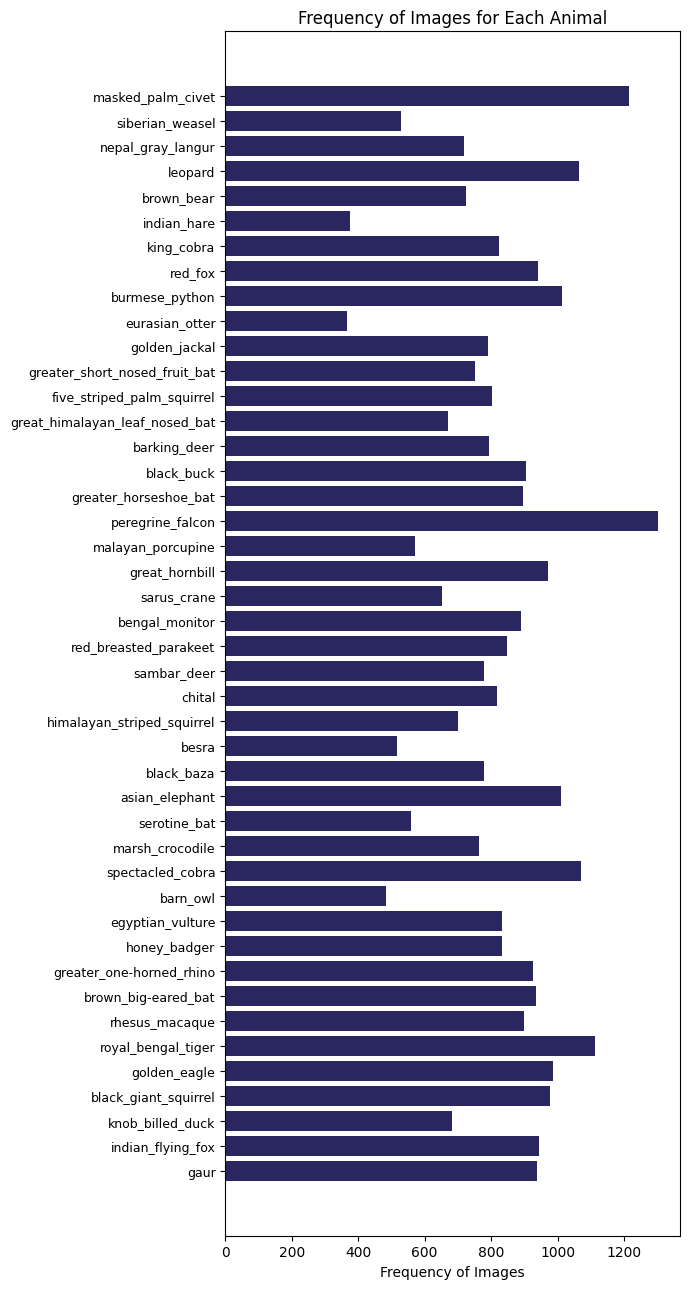
\includegraphics[scale=0.5]{Graphics/naturalist_horizontal.png}
	\caption{Image File count for each animal}
	\label{image-file-count-animal}
\end{figure}




\subsection{Audio Data from Xeno-canto}
Xeno-canto is a website dedicated to sharing wildlife sounds from all over the world. It provides its data under several licenses derived from Creative Commons licenses which are free for use for educational and research purposes. We collected a total of thousands of audio spanning 23 classes and performed temporal segmentation with each segment being 5 seconds long. A total of 16,230 audio files each of 5 sec was now our final dataset. Of the 16,230 audio files, 30 files for each class were used as the test dataset.
API provided by Xeno-canto was used for downloading the data. The bar chart in Figure \ref{audio-file-count-bird} shows the frequency of each class of audio.

	{

		\begin{figure}
			\centering
			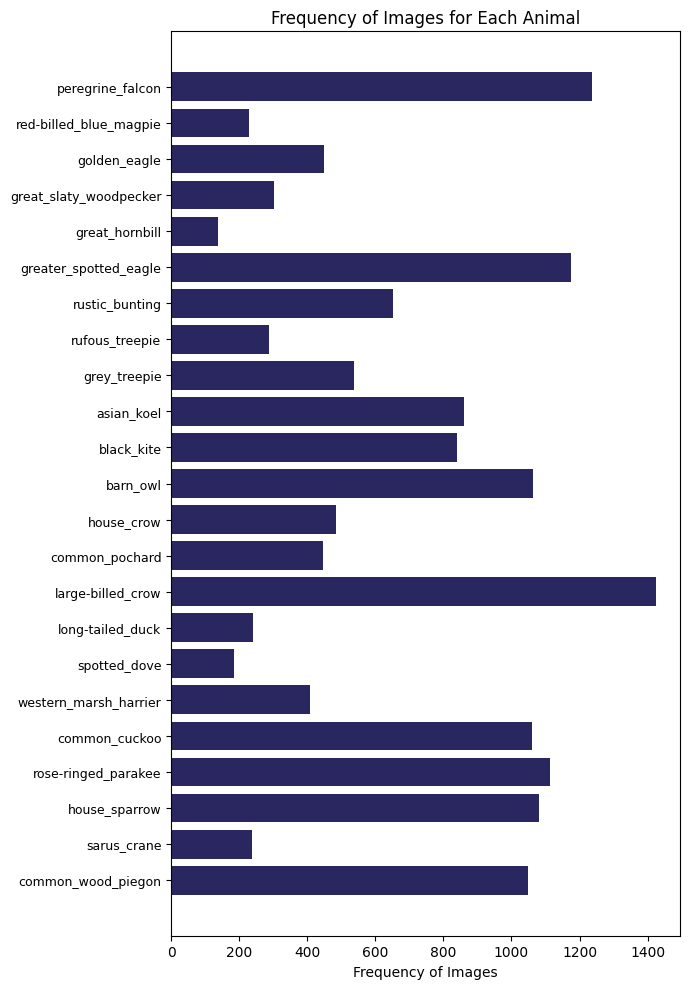
\includegraphics[scale=0.5]{Graphics/xenocanto.png}
			\caption{Audio File count for each bird}
			\label{audio-file-count-bird}
		\end{figure}

	}
\section{Proposed Methodology}
\subsection{Mel-frequency cepstrum Coefficients based on DCT-II for Audio Feature Extraction
}
Mel-frequency cepstrum (MFC) refers to the short-term power spectrum of a sound
based on cosine transform. Mel-frequency cepstrum Coefficients(MFCCs) are coefficients that collectively make up an MFC. Mel-frequency cepstrum Coefficients transform is done on the audio to extract a small set of features that describes our audio.
MFCC helps us to capture the essential spectral characteristics of speech signals in a
compact form, making them suitable for pattern recognition tasks.
\begin{lstlisting}[style=mystyle,caption={MFCC Transformation Function},captionpos=b]
def mfcc_transform(y: np.ndarray,
                   sr: int,
                   mfcc_params: Dict
                   ) -> torch.Tensor:
    melspec = librosa.feature.melspectrogram(
        y=y,
        sr=sr,
        n_fft=mfcc_params['n_fft'],
        win_length=mfcc_params['win_length'],
        hop_length=mfcc_params['hop_length'],
        n_mels=mfcc_params['n_mels'],
        htk=mfcc_params['htk'],
        norm=mfcc_params['norm_melspec'],
    )
    mfcc_librosa = librosa.feature.mfcc(
        S=librosa.core.spectrum.power_to_db(melspec),
        n_mfcc=mfcc_params['n_mfcc'],
        dct_type=mfcc_params['dct_type'],
        norm=mfcc_params['norm_mfcc']
    )

    return torch.from_numpy(mfcc_librosa)
\end{lstlisting}

\subsection{Expansion and Interpolation of Audio Data}
After MFCC transformation, the tensors are transformed again to proper dimension as required by EfficientNetB0 architecture. Following steps are performed:
\begin{itemize}
	\item The input tensor y is replicated along one dimension to create three copies, preparing it for subsequent operations.
	\item The expanded tensor is resized to a fixed size of (224, 224) using bilinear interpolation, ensuring consistent dimensions for neural network input.
	\item Any extra dimensions introduced during resizing are removed, returning the tensor to its original shape.
	\item The processed tensor is returned for further use, completing the preprocessing steps commonly applied to image data for deep learning tasks.
\end{itemize}
\begin{lstlisting}[style=mystyle,caption={MFCC Transformation Function},captionpos=b]
def expand_tensor_for_efficient_net(y) -> torch.Tensor:
    input_tensor_expanded = y.expand(3, -1, -1)
    resized_tensor = F.interpolate(input_tensor_expanded.unsqueeze(
        0), size=(224, 224), mode='bilinear', align_corners=False)

    resized_tensor = resized_tensor.squeeze()
    return resized_tensor
\end{lstlisting}

\subsection{Transformation as required by EfficientNetB0 Input Data}
For best results and compatibility, we transformed our data as per the transformation required for EfficientNetB0 architecture.
\begin{lstlisting}[style=mystyle,caption={MFCC Transformation Function},captionpos=b]
ImageClassification(
    crop_size=[224]
    resize_size=[256]
    mean=[0.485, 0.456, 0.406]
    std=[0.229, 0.224, 0.225]
    interpolation=InterpolationMode.BICUBIC
)
\end{lstlisting}

\subsection{Transfer Learning}
Transfer learning is a technique in the field of machine learning where learned parameters on previously trained data are used to learn parameters of new data. This is done to reuse the learned parameters from previous data. Transfer learning is not
only better for performance but also decreases the time required to learn features about
subject in question.

\subsection{EfficientNetB0}
EfficientNet is a convolutional neural network architecture and scaling method that uniformly scales all dimensions of depth/width/resolution using a compound coefficient \cite{r7}.
Unlike conventional practice that arbitrarily scales these factors, the EfficientNet scaling method uniformly scales network width, depth, and resolution with a set of fixed scaling
coefficients.
\par
\subsection{ Convolutional Neural Network}
Convolutional Neural Networks are specialized kind of neural networks for processing
data that has a grid-like topology \cite{r8}. Most machine learning libraries implement cross-correlation rather than conventionally known convolution operations in the realm of Digital
Signal Processing . In conventional multi-layer perceptrons, large number of parameters are required to learn features where as CNN uses filters to stride through whole data using a lesser number of parameters aka parameter sharing.
% CNNs are often applied in large number of computer vision tasks across the industry.

\section{Result and Analysis}

\begin{center}
	\captionof{table}{Overview of Results of Audio and Video Model}
	\begin{tabular}{ |c|c|c| }
		\hline
		Model  & Accuracy & F1 score \\
		\hline
		Vision & 86.1     & 86.12    \\
		\hline
		Audio  & 90.39    & 88.12    \\
		\hline
	\end{tabular}
\end{center}

\subsection{Vision Model}
The vision model was created with EfficientNetB0 as its base for transfer learning. We were able to achieve an accuracy of 86.1\% with an F1-Score of 86.12 on the test dataset. Table \ref{table1} shows the various metrics of the vision model.
\begin{center}
	\captionof{table}{Vision Model Metrics}
	\begin{tabular}{ |c|c|c| }
		\hline
		\textbf{Parameters}      & \textbf{Metrics}          \\
		\hline
		Batch Size               & 32                        \\
		\hline
		Epochs                   & 10                        \\
		\hline
		Pretrained Model         & EfficientNetB0            \\
		\hline
		Weights                  & ImageNet                  \\
		\hline
		Learning Rate            & 0.0001                    \\
		\hline
		Weight Decay             & 0.001                     \\
		\hline
		Loss Function            & Categorical Cross Entropy \\
		\hline
		Optimizer                & Adam                      \\
		\hline
		Total Parameters         & 4,063,912                 \\
		\hline
		Trainable Parameters     & 4,063,912                 \\
		\hline
		Non-Trainable Parameters & 0                         \\
		\hline
	\end{tabular}
	\label{table1}

\end{center}

The confusion matrix for vision model on the test dataset is shown in Figure \ref{cm_vision}. Figure \ref{accuracy-vision} and Figure \ref{loss-vision} shows the accuracy and loss of vision model respectively.

\begin{figure*}[t] % Use figure* for spanning both columns
	\centering
	\begin{minipage}{\textwidth} % Use minipage to ensure the figure spans the whole width
		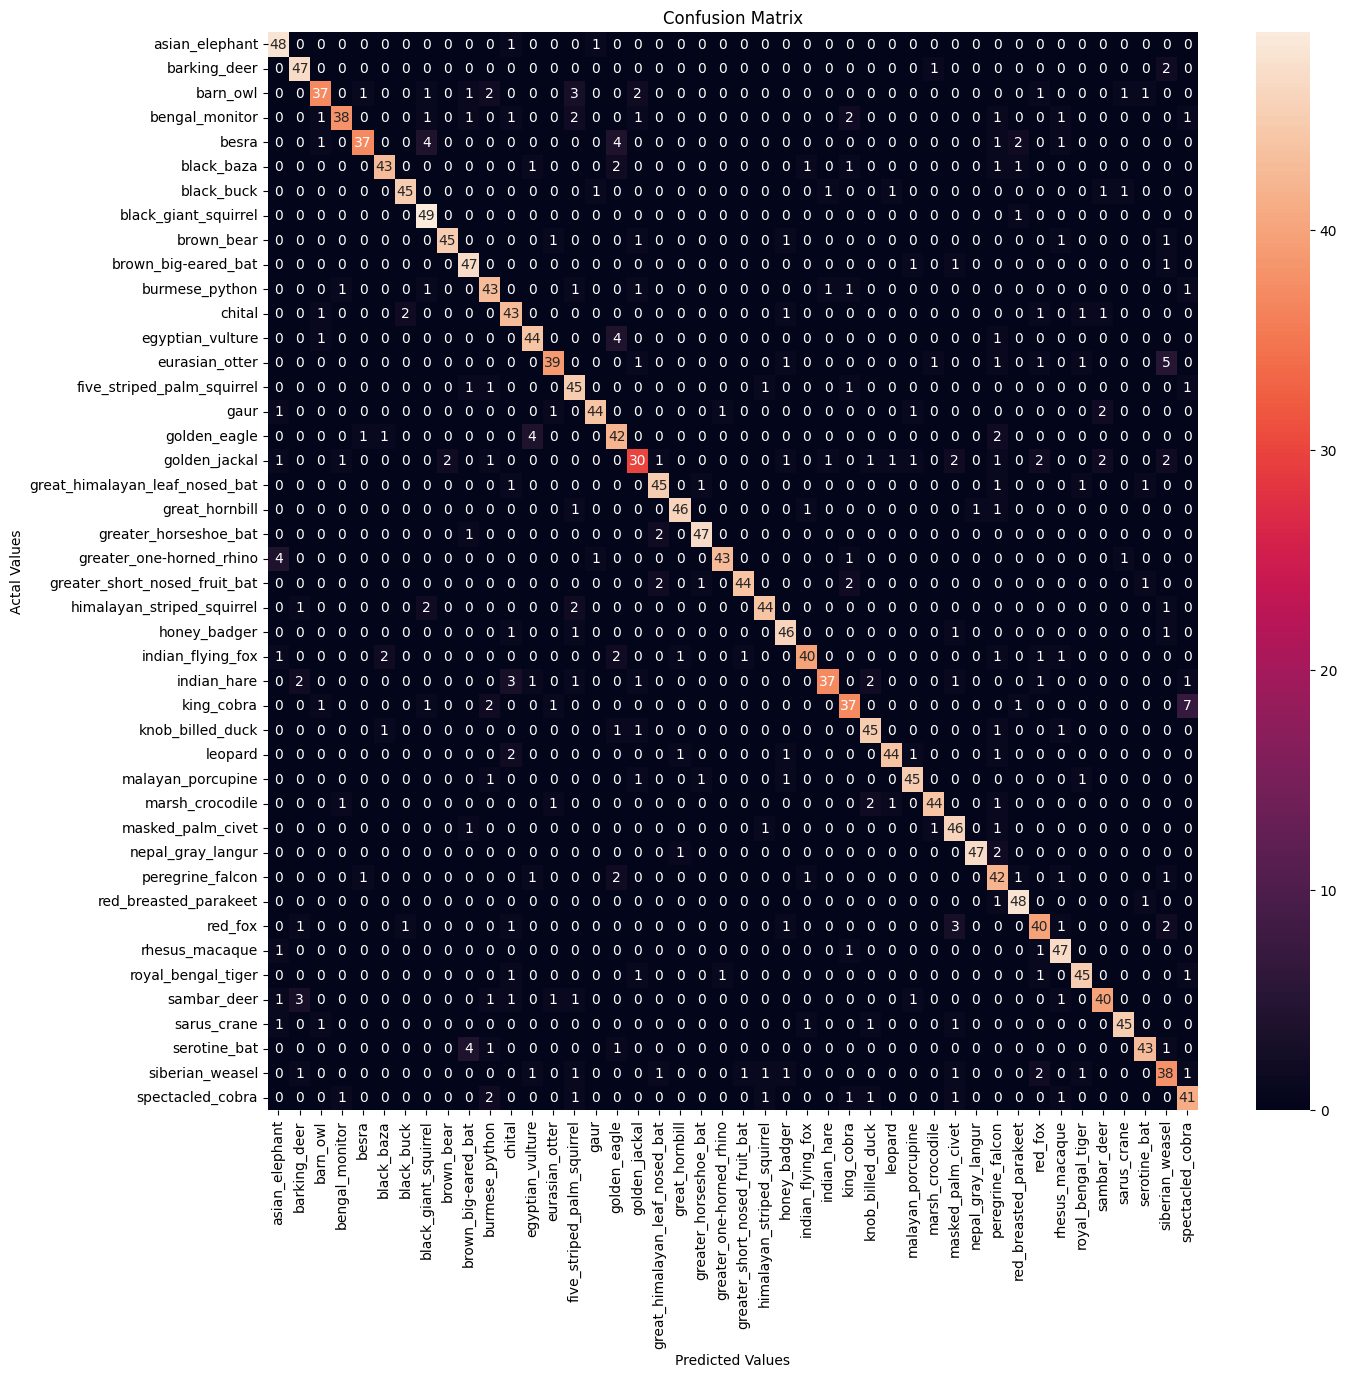
\includegraphics[scale=0.53]{Graphics/vision_cm.png} % Replace example-image with your actual image file
		\caption{Confusion Matrix for Vision Model on test data}
		\label{cm_vision}
	\end{minipage}
\end{figure*}



\begin{figure*}[hbt]
	\centering
	\begin{minipage}[t]{0.45\textwidth}
		\centering
		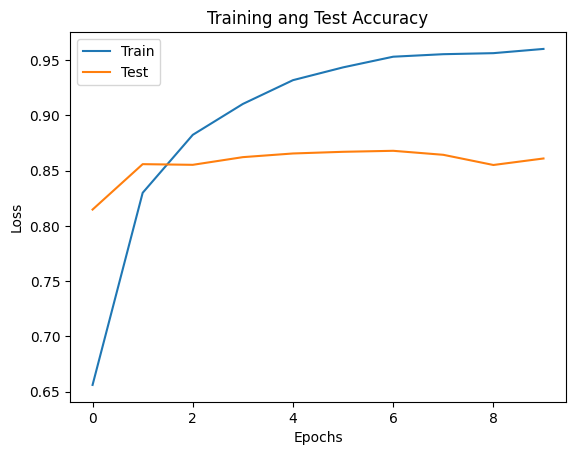
\includegraphics[width=0.8\linewidth]{Graphics/accuracy_vision_model.png}
		\caption{Accuracy of Vision Model on Train and Test Data}
		\label{accuracy-vision}
	\end{minipage}
	\hfill
	\begin{minipage}[t]{0.45\textwidth}
		\centering
		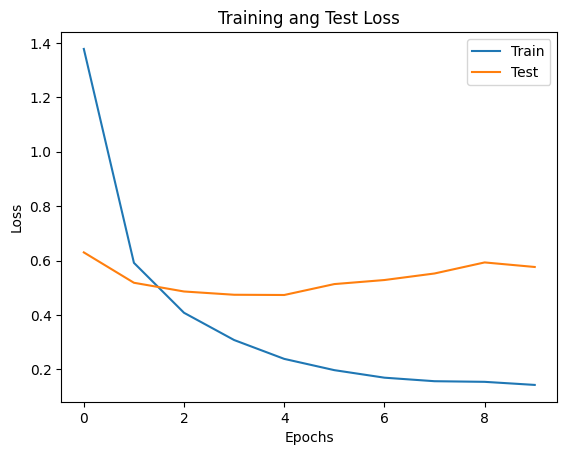
\includegraphics[width=0.8\linewidth]{Graphics/loss_vision.png}
		\caption{Loss of Vision Model on Train and Test Data}
		\label{loss-vision}
	\end{minipage}
\end{figure*}


\clearpage



\subsection{Audio Model}

The audio model was also created with EfficientNetB0 as its base for transfer learning after feature extraction done with MFCC Transform which was again transformed as explained in Section 4.3 for input compatibility with EfficientNetB0.
\par
We were able to achieve an accuracy of 90.39\% and an F1-Score of 88.1 on the test dataset. The batch size of 64 was chosen to increase the training pace. The size of test size of each class is 30.
\par
The following table shows various metrics of the audio model:

\begin{center}
	\captionof{table}{Audio Model Metrics}
	\begin{tabular}{ |c|c|c| }
		\hline
		\textbf{Parameters}      & \textbf{Metrics}          \\
		\hline
		Batch Size               & 64                        \\
		\hline
		Epochs                   & 15                        \\
		\hline
		Pretrained Model         & EfficientNetB0            \\
		\hline
		Weights                  & ImageNet                  \\
		\hline
		Learning Rate            & 0.0001                    \\
		\hline
		Weight Decay             & 0                         \\
		\hline
		Loss Function            & Categorical Cross Entropy \\
		\hline
		Optimizer                & Adam                      \\
		\hline
		Total Parameters         & 4,037,011                 \\
		\hline
		Trainable Parameters     & 4,037,011                 \\
		\hline
		Non-Trainable Parameters & 0                         \\
		\hline
	\end{tabular}
\end{center}
We see a similar pattern as seen in the vision model. Here too in the audio model with similar featured data being mislabeled. Figure \ref{accuracy-audio} and Figure \ref{loss-audio} shows the accuracy and loss of audio model respectively on test data. Figure \ref{cm_audio} shows confusion matrix for audio model on test dataset.


\begin{figure*}[hbt]
	\centering
	\begin{minipage}[t]{0.45\textwidth}
		\centering
		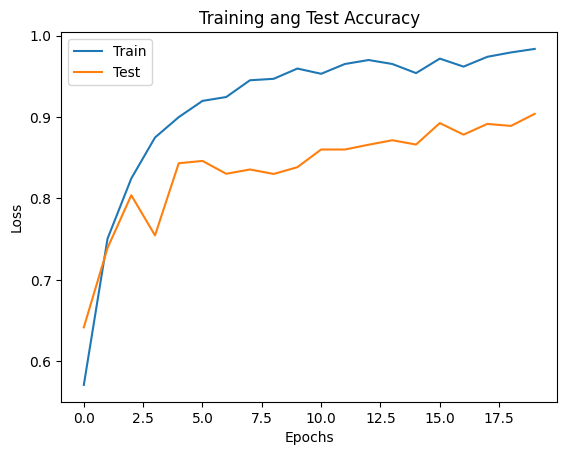
\includegraphics[width=0.8\linewidth]{Graphics/audio_accuracy.png}
		\caption{Accuracy of Audio Model on Train and Test Data}
		\label{accuracy-audio}
	\end{minipage}
	\hfill
	\begin{minipage}[t]{0.45\textwidth}
		\centering
		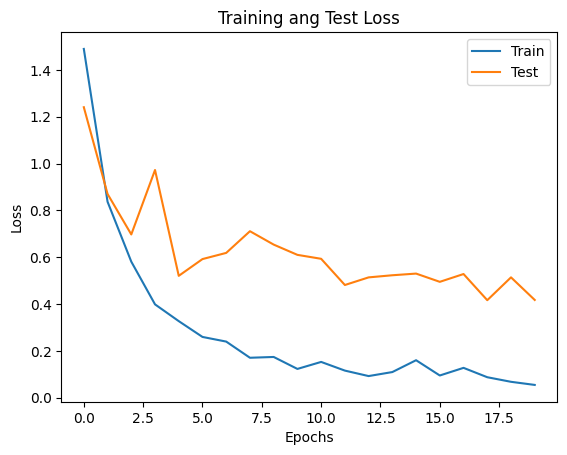
\includegraphics[width=0.8\linewidth]{Graphics/audio_loss.png}
		\caption{Loss of Audio Model on Train and Test Data}
		\label{loss-audio}
	\end{minipage}
\end{figure*}

\begin{figure*}[t] % Use figure* for spanning both columns
	\centering
	\begin{minipage}{\textwidth} % Use minipage to ensure the figure spans the whole width
		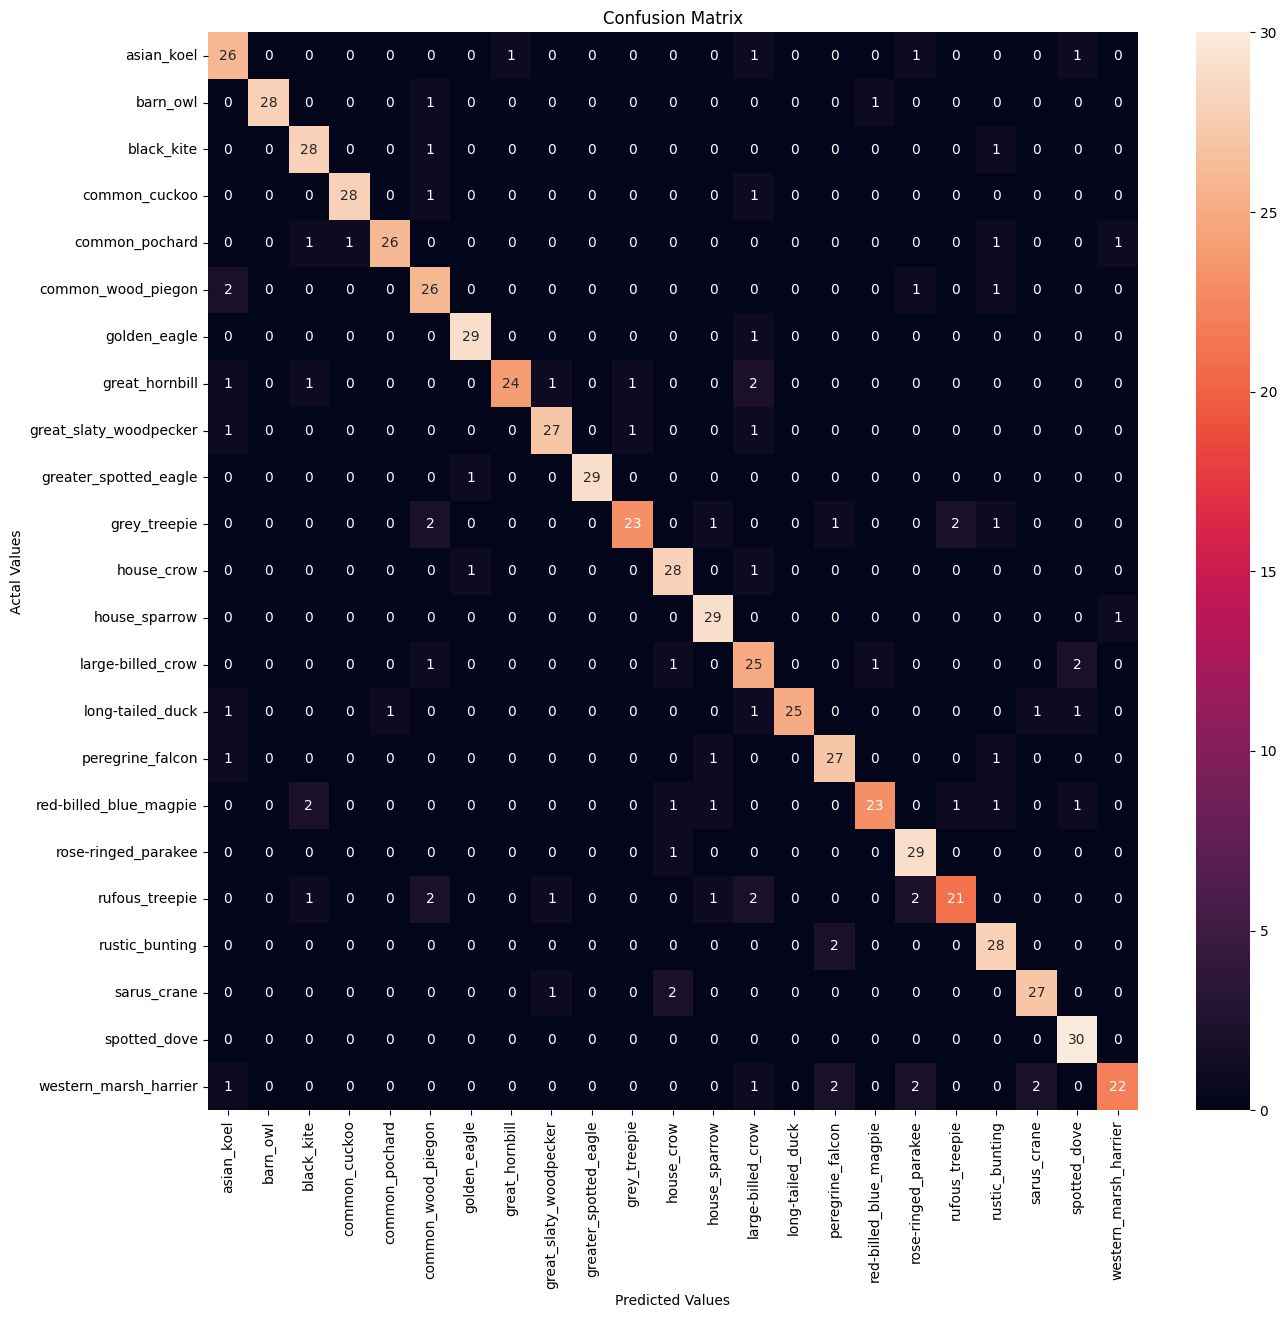
\includegraphics[scale=0.4]{Graphics/audio_cm.png} % Replace example-image with your actual image file
		\caption{Confusion Matrix for Audio Model on test data}
		\label{cm_audio}
	\end{minipage}
\end{figure*}


\section{Conclusion}
Our research work in wildlife classification combines audio and visual technologies, showing promising accuracy levels of 90.39\% and 86.1\% for audio and vision models, respectively. Despite challenges in distinguishing similar species, our study represents a significant advancement in leveraging technology for wildlife conservation. By enhancing monitoring capabilities, we aim to contribute to sustainable conservation practices and promote harmonious coexistence between humans and wildlife.



\phantomsection
\section*{Acknowledgments}
\addcontentsline{toc}{section}{Acknowledgments}
The authors would like to express their gratitude to everyone who supported
them throughout this project. The authors are thankful for their aspiring guidance,
invaluably constructive criticism, and friendly advice during the project work. The authors are
grateful to them for sharing their views on issues related to the project. Without the aid
of our friends and family members, our project would not have been attainable. This
feat would not have been achieved without their assistance.


\phantomsection

\bibliographystyle{unsrt}
\bibliography{references}

\vfill\null
\end{document}
